\documentclass[a4paper, 12pt]{article}
\usepackage[T1]{fontenc}
\usepackage[english]{babel}
\usepackage{hyperref}
\usepackage{enumerate}
\usepackage{graphicx}
\hypersetup{colorlinks=true, linkcolor=blue, filecolor=blue, pagecolor=blue, urlcolor=blue}
\usepackage[normalem]{ulem}
\usepackage{graphicx}
\usepackage{caption}
\usepackage{subcaption}
\usepackage{amsmath}


\begin{document}
\title{\textbf{``Vision-Based Reliable Robot Control Using Hand Gestures''}\\
\vspace{1cm} \large Computer Vision Project Report }\vspace{1cm} 
\author{\it{Students} \\Alexey Y. Ozhigov, ID 9018301
                  \\Yashar A. Rezaei, ID 9015132\\
                    \vspace{0.1cm}\\
                     \it{Supervisor}\\
                    Prof. Dr.-Ing. Rainer Herpers}
\date{\today}
\maketitle
\section{Abstract}
...
\section{Introduction}
...
%The topic of the project is controlling a Lego Mindstorm robot using hand gestures with Kinect camera.
%       By applying machine learning algorithm we try to detect different gestures, then using motion analysis techniques to track the target hand.
%       The aim of the project is to create a user-friendly tele-operation interface for Lego.
%       Operator should be able to drive the robot by means of simple hand movements.
%       E.g. rotating an open hand in the plane set by its fingers turns the robot to the left/right, bending the hand down/up increases/decreases the velocity of the robot (see Figure \ref{fig:gesture_images}).\\
%Context of the project is general tele-operation using hand gestures.
%\subsection{Motivation} Human-robot interaction and tele-operation are an active and promising research field which already has useful applications in our daily life, e.g. robotised medical surgery, game industry, smart TVset, military applications (e.g. see \cite{Goodrich}). The main advantage of such operation is more flexible and remote control over the object.
%\subsection{Objective and Abstract Goal} Software library and simple GUI for Lego Mindstorm NXT tele-operation. Abstract goal is learning CV aspects of human-robot interaction.
%\subsection{Problem Analysis} 
%Tele-operation using hand gestures is a complex problem. Major difficult subproblems are robust gesture recognition, accurate hand pose estimation and hand motion tracking. We simplify the problem by making the the assumptions mentioned in section ``Assumptions and Limitations''.
\section{Assumptions and Limitations}
...
%\textbf{Scenario assumption}
%\begin{itemize}
%\item[1)] Daylight indoor illumination.
%\item[2)] Static background.
%\item[3)] Working range of the hand: from 1m to 2m from the camera.
%\item[4)] Allowed gestures: fist (1) and open hand with spread fingers (2)
%\item[5)] Hand image projection is restricted to a predefined working area during the operation
%\item[6)] Hand bending angle range: from $90^{\circ}$ (min. robot speed) to $45^{\circ}$ (max. robot speed)
%\end{itemize}
%\textbf{Hardware prerequisites}
%\begin{itemize}
%\item[1)] Kinect RGBD camera.
%\item[2)] Modern (for 2012) PC with Bluetooth adapter.
%\item[3)] Lego Mindstorm NXT, standard configuration with Bluetooth module.
%\end{itemize}
%\textbf{Software prerequisites}
%\begin{itemize}
%\item[1)] Programming language(-s) for implementation: C++ and/or Python.
%\end{itemize}
\section{Approach}
This section contains description of the hand tracking algorithm.\\
The algorithm consists of the following steps, each of which is applied to every RGB image and corresponding range image of the input video:
\begin{enumerate}
\item Initialization1. RGB image is converted to gray scale and the palm of the hand is detected by Haar cascade classifier \cite{Viola01} (result: center of the palm, ${P_c}$)
\item Initialization2. RGB image is converted to HSV colour space and Hue histogram at the area around $P_c$ is calculated (result: Hue histogram of the hand skin, $H_c$)
\item Tracking1. RGB image is converted to gray scale and the palm of the hand is detected by Haar cascade classifier (result: current center of the palm, ${P_{c_t}}$)
\item Tracking2. Range image is thresholded using
    \[
        Range_{min} = {P_{c_t}}-50[mm],  \\
        Range_{max} = {P_{c_t}}+50[mm]
    \]
\item Tracking3. CAMSHIFT tracking algorithm is applied to the Hue channel of HSV image with Hue histogram $H_c$ and initial window position returned by Initialization1 step (result: 
\item Tracking4. Since neither the cascade classifier, nor CAMSHIFT
\end{enumerate}
%Haar cascade classifier will be used to distinguish between gestures (1) and (2) (see \cite{Chen}).\\
%Color blob detection and/or 3D depth shareholding will be used to detect hand silhouette. Finger tips on the silhouette will be detected using k-curvature (see \cite{Segen}) algorithm. Rotation of the hand will be detected by measuring angle between line(-s) connecting finger tip(-s) with the center of the hand and vertical line on a 2D image. Bending of the hand will be detected by the hight of the hand bounding box and/or depth values of finger tips.
%\begin{figure}
%        \centering
%        
%        ~ %add desired spacing between images, e. g. ~, \quad, \qquad etc. 
%          %(or a blank line to force the subfigure onto a new line)
%         \begin{subfigure}[b]{0.18\textwidth}
%                          \centering
%                          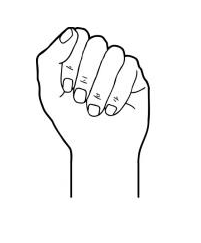
\includegraphics[width=\textwidth]{fist}
%                          \caption{Fist}
%
%                  \end{subfigure}%
%        \begin{subfigure}[b]{0.18\textwidth}
%                \centering
%                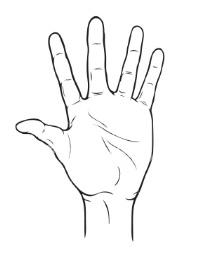
\includegraphics[width=\textwidth]{handopen}
%                \caption{Open hand (initial pose)}
%
%        \end{subfigure}
%        \\
%        \begin{subfigure}[b]{0.2\textwidth}
%                        \centering
%                        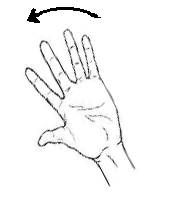
\includegraphics[width=\textwidth]{handleft}
%                        \caption{Rotate left}
%
%                \end{subfigure}
%       \begin{subfigure}[b]{0.21\textwidth}
%                        \centering
%                        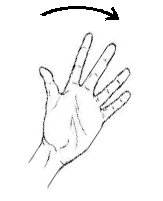
\includegraphics[width=\textwidth]{handright}
%                        \caption{Rotate right}
%
%                        \end{subfigure}
%        \begin{subfigure}[b]{0.25\textwidth}
%                        \centering
%                        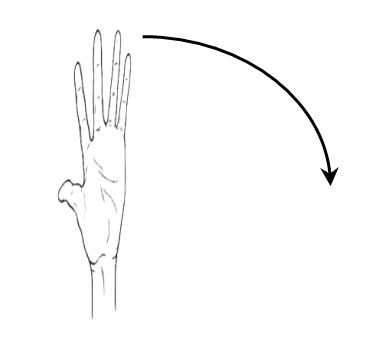
\includegraphics[width=\textwidth]{bendtofront}
%                        \caption{Bend down}
%
%                \end{subfigure}
%        \caption{Sample hand images: a) fist to stop motion, b) initial position (bottom), c) rotating left (upper left),  d) rotating hand right (upper right), e) bending hand down for acceleration (taken from \url{http://www.istockphoto.com})}\label{fig:gesture_images}
%\end{figure}
\section{Alternative approach}
This section describes alternative approach to hand tracking. It does not require cascade classifier and relies on hand contour k-curvature \cite{Segen} analysis to detect the hand. The algorithm steps are the following.
\begin{enumerate}
\item Range thresholding. Assuming the hand is the closest to the camera object, threshold the range image using
    \[
        Range_{min} = 0,  \\
        Range_{max} = {P_{c_t}}+15[cm]
    \] (result: the hand silhouette, $S$)
\item Get the bounding box of $S$ (result: bounding box around the hand, $B$ and its center $B_c$ and height $B_h$). Given the initial height $B_{h_0}$ it is possible to calculate current tilt position $B_{h_t}$ in percents as 
\[
B_{h_t} = B_h / B_0 \cdot 100\%
\]. Driving speed of the robot is proportional to $100-B_{h_t}$ (see Figure \ref{fig:fore}).

\item Get the contour of $S$ (result: contour ${C} = \{C_1, C_2, ..., C_n\}$, a set of points which correspond to the boundary pixels of the silhouette)
\item k-curvature analysis
    \begin{enumerate}
        \item Break $S$ into segments of length $S_{delta}$ ($S_{delta} = 50 [pixels]$ for average sized hand, 1 metre from the camera) (result: ${S_p} = \{S_{p_1}, S_{p_2}, ..., S_{p_M}\}$, a set of segment points, where $S_{p_i} \in C$)
        \item For every $S_{p_i} \in \{S_{p_1}, S_{p_2}, ..., S_{p_M}, S_{p_1}\}, i = 2..M$ calculate angle $A_{i-1}$ which is built by points $S_{p_{i-2}}$, $S_{p_{i-1}}$ and $S_{p_i}$ (result: $A$, a set of segment angles along $S$)
        \item Find finger tips and valleys. Point $S_i$ is considered a tip or a valley if corresponding segment angle $A_i < 1.3 [rad]$ for middle-sized hand, 1 metre from the camera (result: an unordered set of points corresponding to finger tips and valleys, $Q$)
        \item $Q_i$ is considered a tip if 
\[
dist(T_i, B_c) > B_h / 3,
\]
where $dist$ is Euclidean distance (result: a set of points corresponding to finger tips, $T$)
    \end{enumerate}
\item Hand recognition. $S$ is considered a hand if 
\[
5 <= \left|T\right| <= 15
\] i.e. if at least 5 fingers could be detected, but not more than 15. There could be more than 5 fingers detected if the data from which $S$ is obtained is noisy. \\
Test statistics of tips number for sample of size 100 shows $\mu = 7.53$ and $\delta = 1.51$ when images depicted an open hand. For a fist the corresponding values are $\mu = 3.26$ and $\delta = 1.53$.
\item Finding the line segment connecting point and thumb fingers, $L$. If the hand is recognized, a convex hull is calculated from $S$ along with convexity defects. Convexity defect is characterized by depth (how far it is from the contour) and length (see Figure \ref{fig:cont}). Selection criteria for $L$ among other segments of the convex hull is the following: 
\[
    length(L) > 0.6 \cdot B_h \land depth(D_l) > 0.4 \cdot length(L),
\]
where $D_l$ is convexity defect corresponding to $L$. (Result: thumb/point fingers line $L$)
\item Calculate turning angle. Measure angle between $L$ and horizontal line (result: turning angle $\beta$). Given the initial turning angle $\beta_0$, it is possible to get current orientation 
\[
\beta_t = \beta_0 - \beta
\]

\end{enumerate}

\begin{figure}
        \centering
        \includegraphics[width=\textwidth]{cont}
        \caption{Hand contour and convex hull segment between thumb and point fingers}
        \label{fig:cont}
\end{figure}
\begin{figure}
        \centering
        \includegraphics[width=\textwidth]{fore}
        \caption{Hand silhouette with bounding boxes: initial (larger) and current (smaller)}
        \label{fig:fore}
\end{figure}


\section{Evaluation}
...
%The following test scenario will be used to test the performance of the library.
%Human operator puts his hand in front of the camera (gesture (2)) so that the plane of the hand is approximately perpendicular to the optical axis and its outline is confined within a rectangular working area depicted on the screen of the PC. When the hand is detected by the library, corresponding message is displayed on the PC's screen. The operator then bends the hand down and back and rotates it smoothly in the plane of the hand. Any part of the hand image should not move outside the allowed working rectangle.\\
%Possible evaluation task will be navigating the NXT robot along the specified path (e.g. drive 1 meter forward, then turn right, then move 2 meters forward). Navigating should be performed by user with no previous experience with the interface
%Possible issues:
%\begin{itemize}
%\item The hand is occluded from the camera by other objects or there are other objects with the same color as the hand within the working rectangular;
%\item The hand moves outside of the working rectangular;
%\item Lighting conditions change in such a way that the hand gestures and finger tracking cannot be performed accurately with predefined color model for the hand;
%\item The planar shape of the hand gesture (2) is not maintained quite precisely affecting estimation of the angles.
%\end{itemize}

\bibliographystyle{alpha}
\bibliography{bib}
\end{document}
